\scanpage{72}
\mspage{\handwritten{\raisebox{0.65ex}{-}\,7\,-}}

p.25, li.10 du bas : hint pour ``il n'est pas difficile de montrer ...''?

p.26, li.10 : ``dont on peut penser que c'est le même ...'' : y a-t-il \inserted{\parbox[b]{.94\linewidth}{\figure{%
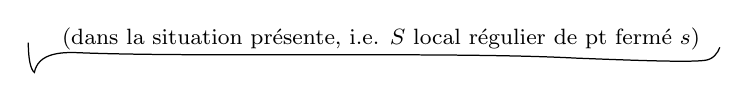
\begin{tikzpicture}
\node[anchor=base west,inner sep=0pt,font=\footnotesize] (addition) at (0,0)
{(dans la situation présente, i.e. $S$ local régulier de pt fermé $s$)};
\handwritten{\draw[line width=0.45pt]
([xshift=-1.20em,yshift=0.65ex]addition.south west)
.. controls ([xshift=-1.20em,yshift=-0.70ex]addition.south west)
and ([xshift=-1.12em,yshift=-1.60ex]addition.south west)
.. ([xshift=-0.98em,yshift=-1.85ex]addition.south west)
.. controls ([xshift=-0.85em,yshift=-0.35ex]addition.south west)
and ([xshift=-0.15em,yshift=-0.10ex]addition.south west)
.. ([xshift=0.65em,yshift=-0.20ex]addition.south west)
.. controls ([xshift=5.0em,yshift=-0.60ex]addition.south west)
and ([xshift=-9.0em,yshift=-0.10ex]addition.south east)
.. ([xshift=-4.5em,yshift=-0.65ex]addition.south east)
.. controls ([xshift=-2.3em,yshift=-0.85ex]addition.south east)
and ([xshift=-0.5em,yshift=-1.00ex]addition.south east)
.. ([xshift=0.12em,yshift=-0.85ex]addition.south east)
.. controls ([xshift=0.48em,yshift=-0.78ex]addition.south east)
and ([xshift=0.62em,yshift=-0.20ex]addition.south east)
.. ([xshift=0.70em,yshift=0.25ex]addition.south east);}
\end{tikzpicture}%
}}} une caractérisation d'un homomorphisme (7.17.4.1) ? \handwritten{(${}^1$)}

p.27, li.1 et 2 du bas : ``au-dessus'' et non ``au dessus''. Dire ``dans le normalisé'' au lieu de ``du normalisé''.

p.28 : dans la bibliographie, manque la référence Abhyankar sur la résolution des singularités des surfaces arithmétiques.

\handwritten{(${}^1$) Est-ce que 7.2 ne \unsure{x|se} généralise pas ?}

% Isolated dark point pair in the blank lower-right region; authorship and function unresolved.
\margin{\raisebox{-7.3cm}[0pt][0pt]{\parbox{2mm}{\figure{\unsure{%
\begin{tikzpicture}[x=1mm,y=1mm,baseline=0pt]
\fill (0,0) ellipse[x radius=0.20,y radius=0.17];
\fill (0.52,0.85) ellipse[x radius=0.16,y radius=0.24,rotate=-32];
\end{tikzpicture}%
}}}}}

% archive sheet number: 71
